%%%%%%%%%%%%%%%%%%%%%%%%%%%%%%%%%%%%%%%%%%%%%%%%%%%%%%%%%%%%%%%%%%%%
%% %%	Posterdown PDF class for LaTeX files	 08-JAN-2019
%% %%	For any information please send an e-mail to:
%% %%		brentthonre18@gmail.com (Brent Thorne)
%% %%
%% %%	Initial class provided by:
%% %%		Brent Thorne
%%%%%%%%%%%%%%%%%%%%%%%%%%%%%%%%%%%%%%%%%%%%%%%%%%%%%%%%%%%%%%%%%%%%

\documentclass[article,30pt,extrafontsizes]{memoir}

%utf-8 seems to be important
\RequirePackage[utf8]{inputenc}
\RequirePackage[T1]{fontenc}
\RequirePackage{lmodern}
\RequirePackage{multicol}
\RequirePackage{graphicx}
\RequirePackage{lipsum}
\RequirePackage{blindtext}
\RequirePackage[svgnames,table]{xcolor}
\RequirePackage{tikz}
\RequirePackage[framemethod=tikz]{mdframed}
\RequirePackage{color}
\RequirePackage{geometry}
\RequirePackage{adjmulticol}
\RequirePackage[skins,most,listings,skins]{tcolorbox}


%For kable extra package :)
\RequirePackage{booktabs}
\RequirePackage{longtable}
\RequirePackage{array}
\RequirePackage{multirow}
\RequirePackage{wrapfig}
\RequirePackage{float}
\RequirePackage{colortbl}
\RequirePackage{pdflscape}
\RequirePackage{pagecolor}
\RequirePackage{tabu}
\RequirePackage{threeparttable}
\RequirePackage{threeparttablex}
\RequirePackage[normalem]{ulem}
\RequirePackage{makecell}
\RequirePackage{wrapfig}

%%%%%%%%% COLOURS %%%%%%%%

%Fill/ Line Colours
\definecolor{titlebgcol}{HTML}{0b4545}
\definecolor{columnlinecol}{HTML}{ffffff}
\definecolor{posterbgcol}{HTML}{ffffff}
\definecolor{headerbgcol}{HTML}{0b4545}
\definecolor{headerbordercol}{HTML}{0b4545}

% Text Colours
\definecolor{titletextcol}{HTML}{ffffff}
\definecolor{authortextcol}{HTML}{008080}
\definecolor{affiliationtextcol}{HTML}{FFFFFF}
\definecolor{headertextcol}{HTML}{ffffff}
\definecolor{bodytextcol}{HTML}{000000}
\definecolor{footnotetextcol}{HTML}{ffffff}
\definecolor{citecol}{HTML}{CC0000}
\definecolor{urlcol}{HTML}{008080}
\definecolor{linkcol}{HTML}{008080}

\RequirePackage{hyperref}
\hypersetup{
    colorlinks=true,
    linkcolor=linkcol,
    citecolor=citecol,
    filecolor=magenta,
    urlcolor=urlcol,
}

%For figure and table placement
\RequirePackage{float}
\floatplacement{figure}{H}
\floatplacement{table}{H}

%spacing between figure/ table and caption
\setlength{\abovecaptionskip}{0.4in}
\setlength{\belowcaptionskip}{0.2in}
\captionnamefont{\footnotesize\sffamily\bfseries}
\captiontitlefont{\footnotesize\sffamily}

%define column options
\setlength{\columnseprule}{1pt}
\def\columnseprulecolor{\color{columnlinecol}}

%define section header title features
\setsubsubsecheadstyle{\small\color{headertextcol}\textbf}% Set \section style
\setsecnumformat{}
\def\sectionmark#1{\markboth{#1}{#1}}


%tcolorbox magic from my stack exchange question
\newtcolorbox{myboxstuff}[1][]{code={\parindent=0em},colframe=headerbordercol,left skip=0pt,valign=center,halign=center,fontupper=\Large\bfseries,colupper=headertextcol,boxrule=6pt,sharp corners,colback=headerbgcol, #1}
\newcommand{\mybox}[1]{%
\begin{myboxstuff}
\strut #1
\end{myboxstuff}%
}
\makeheadstyles{MyBox}{
    \setsecheadstyle{\mybox}
}
\headstyles{MyBox}\makepagestyle{MyBox}


%-----------------------------------------------------

\thispagestyle{empty}
\definecolor{light-gray}{gray}{0.9}

%biblatex options
\RequirePackage[sorting=none,backend=biber]{biblatex}
\renewcommand*{\bibfont}{\tiny}
\bibliography{MyLibrary}
\defbibheading{bibliography}[\bibname]{%
\section*{#1}%
\markboth{#1}{#1}}
\AtBeginDocument{%
  \renewcommand{\bibname}{References}
}

%bring in the users information
\author{Author One\textsuperscript{1} Author Two\textsuperscript{2}}
\title{\fontfamily{phv}\selectfont Using posterdown to generate reproducible
conference posters via RMarkdown \textgreater{} Knitr \textgreater{}
Markdown \textgreater{} Pandoc \textgreater{} Latex \textgreater{} PDF
workflow}
\counterwithout{section}{chapter}


\makechapterstyle{mydefault}{
\addtocounter{secnumdepth}{2}
\setsecheadstyle{\mybox}
\setsubsecheadstyle{\itshape}
\setsubsubsecheadstyle{\itshape}
}

\chapterstyle{mydefault}

%define column spacing
\setlength\columnsep{1in}

\setlength\parindent{1em}
\setlength\parskip{1em}
\setlength\hangparas{0}

%spacing after section head title
\setaftersecskip{0.3in}
\setbeforesecskip{1in}
\setlength\textfloatsep{0.3in}
\setlength\floatsep{0.3in}
\setlength\intextsep{0.3in}

\setstocksize{39in}{45in}
\settrimmedsize{\stockheight}{\stockwidth}{*}
\settypeblocksize{39in}{45in}{*}
\setlrmargins{*}{*}{1}
\setulmarginsandblock{2.5cm}{*}{*}
\setmarginnotes{0em}{0cm}{0cm}
\setlength{\footskip}{0cm}
\setlength{\footnotesep}{0cm}
\setlength{\headheight}{0pt}
\setlength{\headsep}{0pt}
\setlength{\trimtop}{0pt}
\setlength{\trimedge}{0pt}
\setlength{\uppermargin}{0pt}
\checkandfixthelayout

\mdfdefinestyle{brentsmdfstyle}{%
  backgroundcolor=titlebgcol,
  linecolor=columnlinecol,
  topline=false,
  leftline=false,
  rightline=false,
  linewidth=2mm}

%Footnote to white
\RequirePackage{footmisc}
\def\footnotelayout{\centering\color{footnotetextcol}}

% see https://stackoverflow.com/a/47122900
\usepackage{color}
\usepackage{fancyvrb}
\newcommand{\VerbBar}{|}
\newcommand{\VERB}{\Verb[commandchars=\\\{\}]}
\DefineVerbatimEnvironment{Highlighting}{Verbatim}{commandchars=\\\{\}}
% Add ',fontsize=\small' for more characters per line
\usepackage{framed}
\definecolor{shadecolor}{RGB}{248,248,248}
\newenvironment{Shaded}{\begin{snugshade}}{\end{snugshade}}
\newcommand{\KeywordTok}[1]{\textcolor[rgb]{0.13,0.29,0.53}{\textbf{#1}}}
\newcommand{\DataTypeTok}[1]{\textcolor[rgb]{0.13,0.29,0.53}{#1}}
\newcommand{\DecValTok}[1]{\textcolor[rgb]{0.00,0.00,0.81}{#1}}
\newcommand{\BaseNTok}[1]{\textcolor[rgb]{0.00,0.00,0.81}{#1}}
\newcommand{\FloatTok}[1]{\textcolor[rgb]{0.00,0.00,0.81}{#1}}
\newcommand{\ConstantTok}[1]{\textcolor[rgb]{0.00,0.00,0.00}{#1}}
\newcommand{\CharTok}[1]{\textcolor[rgb]{0.31,0.60,0.02}{#1}}
\newcommand{\SpecialCharTok}[1]{\textcolor[rgb]{0.00,0.00,0.00}{#1}}
\newcommand{\StringTok}[1]{\textcolor[rgb]{0.31,0.60,0.02}{#1}}
\newcommand{\VerbatimStringTok}[1]{\textcolor[rgb]{0.31,0.60,0.02}{#1}}
\newcommand{\SpecialStringTok}[1]{\textcolor[rgb]{0.31,0.60,0.02}{#1}}
\newcommand{\ImportTok}[1]{#1}
\newcommand{\CommentTok}[1]{\textcolor[rgb]{0.56,0.35,0.01}{\textit{#1}}}
\newcommand{\DocumentationTok}[1]{\textcolor[rgb]{0.56,0.35,0.01}{\textbf{\textit{#1}}}}
\newcommand{\AnnotationTok}[1]{\textcolor[rgb]{0.56,0.35,0.01}{\textbf{\textit{#1}}}}
\newcommand{\CommentVarTok}[1]{\textcolor[rgb]{0.56,0.35,0.01}{\textbf{\textit{#1}}}}
\newcommand{\OtherTok}[1]{\textcolor[rgb]{0.56,0.35,0.01}{#1}}
\newcommand{\FunctionTok}[1]{\textcolor[rgb]{0.00,0.00,0.00}{#1}}
\newcommand{\VariableTok}[1]{\textcolor[rgb]{0.00,0.00,0.00}{#1}}
\newcommand{\ControlFlowTok}[1]{\textcolor[rgb]{0.13,0.29,0.53}{\textbf{#1}}}
\newcommand{\OperatorTok}[1]{\textcolor[rgb]{0.81,0.36,0.00}{\textbf{#1}}}
\newcommand{\BuiltInTok}[1]{#1}
\newcommand{\ExtensionTok}[1]{#1}
\newcommand{\PreprocessorTok}[1]{\textcolor[rgb]{0.56,0.35,0.01}{\textit{#1}}}
\newcommand{\AttributeTok}[1]{\textcolor[rgb]{0.77,0.63,0.00}{#1}}
\newcommand{\RegionMarkerTok}[1]{#1}
\newcommand{\InformationTok}[1]{\textcolor[rgb]{0.56,0.35,0.01}{\textbf{\textit{#1}}}}
\newcommand{\WarningTok}[1]{\textcolor[rgb]{0.56,0.35,0.01}{\textbf{\textit{#1}}}}
\newcommand{\AlertTok}[1]{\textcolor[rgb]{0.94,0.16,0.16}{#1}}
\newcommand{\ErrorTok}[1]{\textcolor[rgb]{0.64,0.00,0.00}{\textbf{#1}}}
\newcommand{\NormalTok}[1]{#1}

% choose font family
\RequirePackage{palatino}

\newpagecolor{posterbgcol}

%begin the document
\begin{document}

\begin{mdframed}[style=brentsmdfstyle]

%sets footnote to be white hopefully
\renewcommand\footnoterule{}
\renewcommand{\thempfootnote}{\footnotesize\color{footnotetextcol}{\arabic{mpfootnote}}}

% group which adds title author and other infor
% Used instead of \maketitle for better spacing options
\begingroup
  \centering
  \color{titletextcol}
\vspace{0.5in}
  \Huge{\fontfamily{phv}\selectfont Using posterdown to generate reproducible
conference posters via RMarkdown \textgreater{} Knitr \textgreater{}
Markdown \textgreater{} Pandoc \textgreater{} Latex \textgreater{} PDF
workflow}  \\[0.3in]
  \color{authortextcol} \Large{Author One\textsuperscript{1} Author Two\textsuperscript{2}} \\[0.2in]
  \color{affiliationtextcol} \large{\textsuperscript{1}Department of Poster Layouts, University of Markdown;
\textsuperscript{2}Deparment of Another Institution, Institution
University}
  \vspace{0.2in}

% end title section -------------------
  \endgroup
\end{mdframed}

% Brgin body of poster
\begin{adjmulticols*}{4}{10mm}{10mm}
\normalsize{
\color{bodytextcol}
\section{Introduction}\label{introduction}

Welcome to \texttt{posterdown} ! This is my attempt to provide a
semi-smooth workflow for those who wish to take their \texttt{RMarkdown}
skills to the conference world. Many creature comforts from
\texttt{RMarkdown} are available in this package such as
\texttt{Markdown} section notation, figure captioning, and even
citations like this one \autocite{holden_identifying_2012} The rest of
this example poster will show how you can insert typical conference
poster features into your own document.

\section{Study Site}\label{study-site}

Here is a map made to show the study site using \texttt{ggplot2},
\texttt{ggspatial}, and \texttt{sf}. Lorem ipsum dolor sit amet,
\autocite{middleton_geological_nodate} consectetur adipiscing elit, sed
do eiusmod tempor incididunt ut labore et dolore magna aliqua. Phasellus
vestibulum lorem sed risus ultricies tristique nulla. Mauris vitae
ultricies leo integer malesuada nunc vel risus commodo. Suspendisse
potenti nullam ac tortor vitae. Enim nunc faucibus a pellentesque sit
amet porttitor eget.

\begin{figure}

{\centering 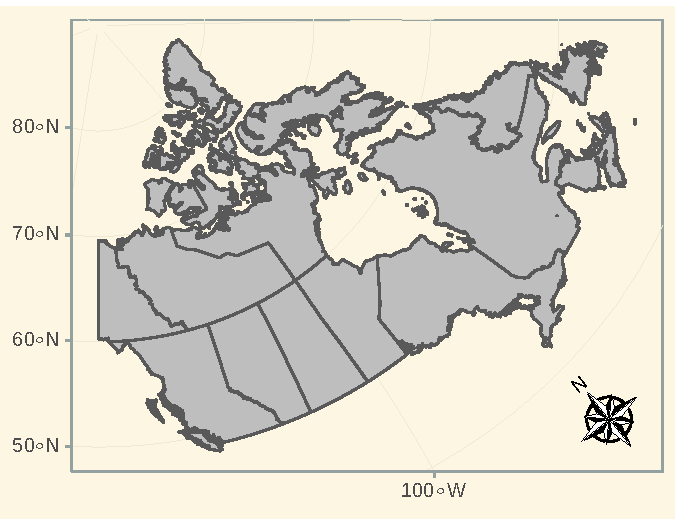
\includegraphics[width=0.8\linewidth]{skeleton_files/figure-latex/unnamed-chunk-2-1} 

}

\caption{This is a map of Canada, the ggspatial package is great for GIS folks in R!}\label{fig:unnamed-chunk-2}
\end{figure}

\section{Objectives}\label{objectives}

\large

\begin{enumerate}
\def\labelenumi{\arabic{enumi}.}
\tightlist
\item
  Easy to use reproducible poster design.
\item
  Integration with \texttt{RMarkdown}.
\item
  Easy transition from \texttt{posterdown} to \texttt{thesisdown} or
  \texttt{rticles}
\end{enumerate}

\small

\section{Methods}\label{methods}

This package uses the same workflow approach as the \texttt{RMarkdown}
you know and love. Basically it goes from RMarkdown \textgreater{} Knitr
\textgreater{} Markdown \textgreater{} Pandoc \textgreater{} Latex
\textgreater{} PDF

\lipsum[1-3]

\section{Results}\label{results}

Usually you want to have a nice table displaying some important results
that you have calcualated. In posterdown this is as easy as using the
\texttt{kable} table formatting you are probably use to as per typical
\texttt{RMarkdown} formatting. I suggesting checking out the
\texttt{kableExtra} package and its in depth documentation on
customizing these tables found
\href{https://haozhu233.github.io/kableExtra/awesome_table_in_pdf.pdf}{here}.

\vspace{1in}

\begin{table}[H]

\caption{\label{tab:unnamed-chunk-3}Tables are a breeze with Kable and Kable extra package!}
\centering
\fontsize{25}{27}\selectfont
\begin{tabu} to \linewidth {>{\centering}X>{\centering}X>{\centering}X>{\centering}X>{\centering}X}
\toprule
Sepal.Length & Sepal.Width & Petal.Length & Petal.Width & Species\\
\midrule
\rowcolor{gray!6}  5.1 & 3.5 & 1.4 & 0.2 & setosa\\
4.9 & 3.0 & 1.4 & 0.2 & setosa\\
\rowcolor{gray!6}  4.7 & 3.2 & 1.3 & 0.2 & setosa\\
4.6 & 3.1 & 1.5 & 0.2 & setosa\\
\bottomrule
\end{tabu}
\end{table}

\begin{figure}

{\centering 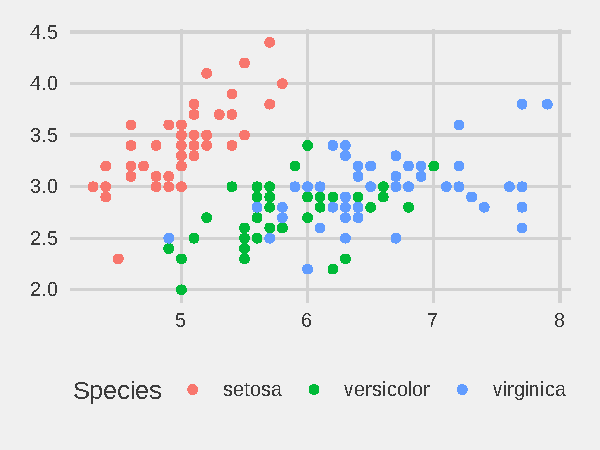
\includegraphics[width=0.75\linewidth]{skeleton_files/figure-latex/unnamed-chunk-4-1} 

}

\caption{A typical plot using ggplot using the classic iris dataset.}\label{fig:unnamed-chunk-4}
\end{figure}

\begin{figure}

{\centering 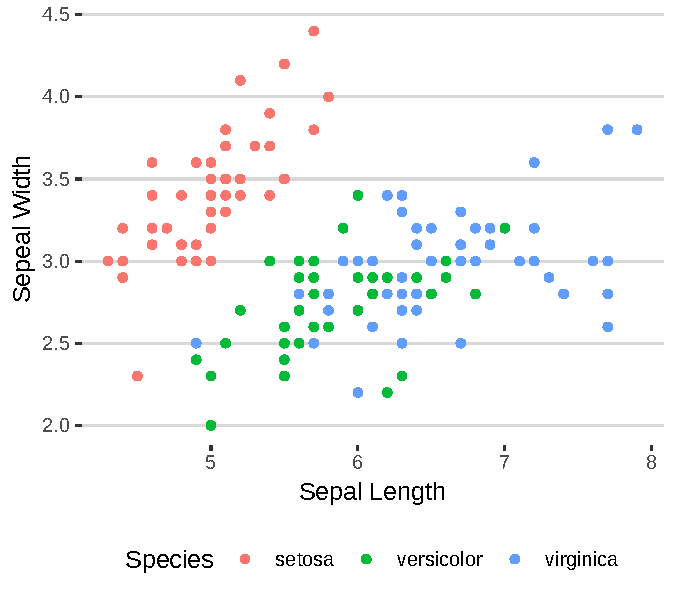
\includegraphics[width=0.85\linewidth]{skeleton_files/figure-latex/unnamed-chunk-5-1} 

}

\caption{Another typical plot using ggplot, this time with a different theme and r code chunk options for fig.width and fig.height.}\label{fig:unnamed-chunk-5}
\end{figure}

\begin{Shaded}
\begin{Highlighting}[]
\CommentTok{# Here is some code for people}
\CommentTok{# to look at and be in awe of!!!!}
\KeywordTok{library}\NormalTok{(ggplot2)}
\KeywordTok{library}\NormalTok{(ggthemes)}

\KeywordTok{ggplot}\NormalTok{(}\DataTypeTok{data=}\NormalTok{iris,}
       \KeywordTok{aes}\NormalTok{(}\DataTypeTok{x =}\NormalTok{ Sepal.Width,}
           \DataTypeTok{y =}\NormalTok{ Sepal.Length,}
           \DataTypeTok{colour =}\NormalTok{ Species)) }\OperatorTok{+}
\StringTok{  }\KeywordTok{geom_point}\NormalTok{() }\OperatorTok{+}
\StringTok{  }\KeywordTok{theme_stata}\NormalTok{() }\OperatorTok{+}
\StringTok{  }\OtherTok{NULL}
\end{Highlighting}
\end{Shaded}

\begin{figure}

{\centering 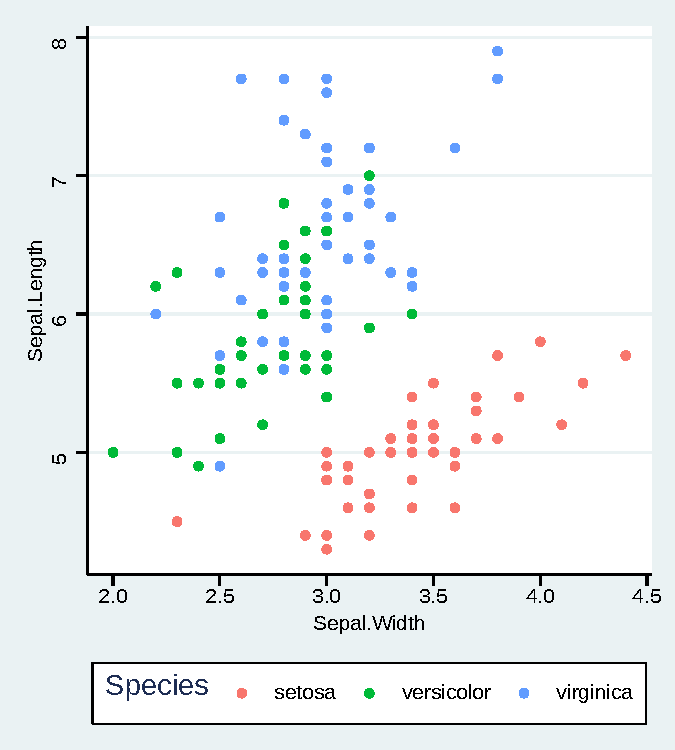
\includegraphics[width=0.8\linewidth]{skeleton_files/figure-latex/unnamed-chunk-6-1} 

}

\caption{Another figure showing how base R plots might look on this poster!}\label{fig:unnamed-chunk-6}
\end{figure}

\lipsum[1-5]

\section{Next Steps}\label{next-steps}

There is still \textbf{A LOT} of work to do on this package which
include (but are note limited to):

\begin{itemize}
\tightlist
\item
  Better softcoding for front end user options in YAML
\item
  Images in the title section for logo placement which is a common
  attribut to posters as far as I have come to know.
\item
  Figure out compatiability with \texttt{natbib} which wasn't working
  during the initial set up.
\item
  MUCH BETTER PACKAGE DOCUMENTATION. For example, there is nothing in
  the README\ldots{}
\item
  Include References section only if initiated by the user like in
  RMarkdown.
\end{itemize}

\small\printbibliography
}
\end{adjmulticols*}
%end the poster
\end{document}
